\documentclass[hyperref={pdfpagelabels=false},professionalfonts,10pt,serif,table,xcolor=dvipsnames]{beamer}

\usepackage{hyperref}
\hypersetup{
	pdfpagelabels=false
}

\usetheme{Warsaw}

\definecolor{darkgreen}{rgb}{0, 0.5, 0.0}
\newcommand{\docutilsrolegreen}[1]{\color{darkgreen}#1\normalcolor}
\newcommand{\docutilsrolered}[1]{\color{red}#1\normalcolor}

\newcommand{\green}[1]{\color{darkgreen}#1\normalcolor}
\newcommand{\red}[1]{\color{red}#1\normalcolor}

\usepackage{lmodern}
%\usepackage{garamond}
\usepackage[garamond]{mathdesign}
%\usepackage[urw-garamond]{mathdesign}

%\usepackage{amsmath}
%\usepackage{amssymb}
%\usepackage{amsthm}
%\usepackage{amsfonts}
\usepackage{graphicx}
\usepackage{verbatim}
\usepackage{fancyvrb}
\usepackage{verbments}
\usepackage{colortbl}
\usepackage{slashed}
\usepackage{tabularx}
%\usepackage[normalem]{ulem}
\usepackage{tikz}

\usepackage[loop, autoplay, buttonsize=1em, buttonbg=0, buttonfg=1]{animate}
\usepackage{movie15}

\providecommand\thispdfpagelabel[1]{}

\usetikzlibrary{shapes,arrows,trees}
\hypersetup{
colorlinks=true,
urlcolor=blue,
linkcolor=blue
}

%\usefonttheme[onlymath]{serif}
%\usecolortheme{orchid}
%\useinnertheme{rounded}

%\setbeamertemplate{headline}[default]
\setbeamercolor{author in head/foot}{fg=black,bg=white}
\setbeamercolor{title in head/foot}{fg=black,bg=white}
\setbeamercolor{date in head/foot}{fg=black,bg=white}

%\addtoheadtemplate{\pgfuseshading{beamer@headfade}\vskip-1.25cm}{}
%\usebackgroundtemplate{\includegraphics[width=\paperwidth,height=\paperheight]{images/bg.eps}}

%\setbeamercolor{frametitle}{bg=Blue,fg=white}
%\setbeamercolor{title}{bg=Blue,fg=white}

%\setbeamersize{text margin left=.2cm} 
%\setbeamersize{text margin right=.5cm}

\setbeamertemplate{itemize itemsep}[0.3in]
\setbeamertemplate{itemize parsep}[0.3in]
\setbeamertemplate{enumerate itemsep}[0.3in]
\setbeamertemplate{enumerate parsep}[0.3in]

\setbeamertemplate{navigation symbols}{}
\setbeamersize{text margin left=.2cm,text margin right=.2cm}
\setbeamercovered{transparent}

\newcommand{\maxFrameImage}[1]
{
	{
	\setbeamercolor{background canvas}{bg=black,fg=white}
	\usebeamercolor[fg]{background canvas}
	\begin{frame}[plain]
	\begin{changemargin}{-1cm}{-1cm}
	\begin{center}
	\includegraphics[width=1.01\paperwidth,height=1.01\paperheight,keepaspectratio]{#1}
	\end{center}
	\end{changemargin}
	\end{frame}
	}
}

\newenvironment{changemargin}[2]{
	\begin{list}{}
	{
	\setlength{\topsep}{-3pt}
	\setlength{\leftmargin}{#1}
	\setlength{\rightmargin}{#2}
	\setlength{\listparindent}{\parindent}
	\setlength{\itemindent}{\parindent}
	\setlength{\parsep}{\parskip}
	}
	\item[]
}{\end{list}}

\newenvironment<>{varblock}[2][\textwidth]
{
	\setlength{\textwidth}{#1}
	\begin{actionenv}#3
	\def\insertblocktitle{#2}
	\par
	\usebeamertemplate{block begin}
	}
	{\pa
	\usebeamertemplate{block end}
	\end{actionenv}
}

\defbeamertemplate*{footline}{my theme}
{
  \leavevmode%
  \hbox{%
  \begin{beamercolorbox}[wd=.333333\paperwidth,ht=3.25ex,dp=1.25ex,left]{author in head/foot}%
    \usebeamerfont{author in head/foot}\hspace*{3.25ex}\insertshortauthor~~(\insertshortinstitute)
  \end{beamercolorbox}%
  \begin{beamercolorbox}[wd=.333333\paperwidth,ht=3.25ex,dp=1.25ex,center]{date in head/foot}%
    \usebeamerfont{date in head/foot}%\insertshortdate{}\hspace*{2em}
    {\large\insertframenumber{}}/\inserttotalframenumber{}
  \end{beamercolorbox}}%
  \begin{beamercolorbox}[wd=.333333\paperwidth,ht=3.25ex,dp=1.25ex,right]{title in head/foot}%
    \usebeamerfont{title in head/foot}\insertshorttitle\hspace*{3.25ex}
  \end{beamercolorbox}%
  \vskip0pt%
}


../common/phys_defs.tex
\usepackage{fancyvrb}
\usepackage{color}
\usepackage[ascii]{inputenc}

\makeatletter
\def\PY@reset{\let\PY@it=\relax \let\PY@bf=\relax%
    \let\PY@ul=\relax \let\PY@tc=\relax%
    \let\PY@bc=\relax \let\PY@ff=\relax}
\def\PY@tok#1{\csname PY@tok@#1\endcsname}
\def\PY@toks#1+{\ifx\relax#1\empty\else%
    \PY@tok{#1}\expandafter\PY@toks\fi}
\def\PY@do#1{\PY@bc{\PY@tc{\PY@ul{%
    \PY@it{\PY@bf{\PY@ff{#1}}}}}}}
\def\PY#1#2{\PY@reset\PY@toks#1+\relax+\PY@do{#2}}

\expandafter\def\csname PY@tok@gd\endcsname{\def\PY@tc##1{\textcolor[rgb]{0.63,0.00,0.00}{##1}}}
\expandafter\def\csname PY@tok@gu\endcsname{\let\PY@bf=\textbf\def\PY@tc##1{\textcolor[rgb]{0.50,0.00,0.50}{##1}}}
\expandafter\def\csname PY@tok@gt\endcsname{\def\PY@tc##1{\textcolor[rgb]{0.00,0.25,0.82}{##1}}}
\expandafter\def\csname PY@tok@gs\endcsname{\let\PY@bf=\textbf}
\expandafter\def\csname PY@tok@gr\endcsname{\def\PY@tc##1{\textcolor[rgb]{1.00,0.00,0.00}{##1}}}
\expandafter\def\csname PY@tok@cm\endcsname{\let\PY@it=\textit\def\PY@tc##1{\textcolor[rgb]{0.25,0.50,0.50}{##1}}}
\expandafter\def\csname PY@tok@vg\endcsname{\def\PY@tc##1{\textcolor[rgb]{0.10,0.09,0.49}{##1}}}
\expandafter\def\csname PY@tok@m\endcsname{\def\PY@tc##1{\textcolor[rgb]{0.40,0.40,0.40}{##1}}}
\expandafter\def\csname PY@tok@mh\endcsname{\def\PY@tc##1{\textcolor[rgb]{0.40,0.40,0.40}{##1}}}
\expandafter\def\csname PY@tok@go\endcsname{\def\PY@tc##1{\textcolor[rgb]{0.50,0.50,0.50}{##1}}}
\expandafter\def\csname PY@tok@ge\endcsname{\let\PY@it=\textit}
\expandafter\def\csname PY@tok@vc\endcsname{\def\PY@tc##1{\textcolor[rgb]{0.10,0.09,0.49}{##1}}}
\expandafter\def\csname PY@tok@il\endcsname{\def\PY@tc##1{\textcolor[rgb]{0.40,0.40,0.40}{##1}}}
\expandafter\def\csname PY@tok@cs\endcsname{\let\PY@it=\textit\def\PY@tc##1{\textcolor[rgb]{0.25,0.50,0.50}{##1}}}
\expandafter\def\csname PY@tok@cp\endcsname{\def\PY@tc##1{\textcolor[rgb]{0.74,0.48,0.00}{##1}}}
\expandafter\def\csname PY@tok@gi\endcsname{\def\PY@tc##1{\textcolor[rgb]{0.00,0.63,0.00}{##1}}}
\expandafter\def\csname PY@tok@gh\endcsname{\let\PY@bf=\textbf\def\PY@tc##1{\textcolor[rgb]{0.00,0.00,0.50}{##1}}}
\expandafter\def\csname PY@tok@ni\endcsname{\let\PY@bf=\textbf\def\PY@tc##1{\textcolor[rgb]{0.60,0.60,0.60}{##1}}}
\expandafter\def\csname PY@tok@nl\endcsname{\def\PY@tc##1{\textcolor[rgb]{0.63,0.63,0.00}{##1}}}
\expandafter\def\csname PY@tok@nn\endcsname{\let\PY@bf=\textbf\def\PY@tc##1{\textcolor[rgb]{0.00,0.00,1.00}{##1}}}
\expandafter\def\csname PY@tok@no\endcsname{\def\PY@tc##1{\textcolor[rgb]{0.53,0.00,0.00}{##1}}}
\expandafter\def\csname PY@tok@na\endcsname{\def\PY@tc##1{\textcolor[rgb]{0.49,0.56,0.16}{##1}}}
\expandafter\def\csname PY@tok@nb\endcsname{\def\PY@tc##1{\textcolor[rgb]{0.00,0.50,0.00}{##1}}}
\expandafter\def\csname PY@tok@nc\endcsname{\let\PY@bf=\textbf\def\PY@tc##1{\textcolor[rgb]{0.00,0.00,1.00}{##1}}}
\expandafter\def\csname PY@tok@nd\endcsname{\def\PY@tc##1{\textcolor[rgb]{0.67,0.13,1.00}{##1}}}
\expandafter\def\csname PY@tok@ne\endcsname{\let\PY@bf=\textbf\def\PY@tc##1{\textcolor[rgb]{0.82,0.25,0.23}{##1}}}
\expandafter\def\csname PY@tok@nf\endcsname{\def\PY@tc##1{\textcolor[rgb]{0.00,0.00,1.00}{##1}}}
\expandafter\def\csname PY@tok@si\endcsname{\let\PY@bf=\textbf\def\PY@tc##1{\textcolor[rgb]{0.73,0.40,0.53}{##1}}}
\expandafter\def\csname PY@tok@s2\endcsname{\def\PY@tc##1{\textcolor[rgb]{0.73,0.13,0.13}{##1}}}
\expandafter\def\csname PY@tok@vi\endcsname{\def\PY@tc##1{\textcolor[rgb]{0.10,0.09,0.49}{##1}}}
\expandafter\def\csname PY@tok@nt\endcsname{\let\PY@bf=\textbf\def\PY@tc##1{\textcolor[rgb]{0.00,0.50,0.00}{##1}}}
\expandafter\def\csname PY@tok@nv\endcsname{\def\PY@tc##1{\textcolor[rgb]{0.10,0.09,0.49}{##1}}}
\expandafter\def\csname PY@tok@s1\endcsname{\def\PY@tc##1{\textcolor[rgb]{0.73,0.13,0.13}{##1}}}
\expandafter\def\csname PY@tok@sh\endcsname{\def\PY@tc##1{\textcolor[rgb]{0.73,0.13,0.13}{##1}}}
\expandafter\def\csname PY@tok@sc\endcsname{\def\PY@tc##1{\textcolor[rgb]{0.73,0.13,0.13}{##1}}}
\expandafter\def\csname PY@tok@sx\endcsname{\def\PY@tc##1{\textcolor[rgb]{0.00,0.50,0.00}{##1}}}
\expandafter\def\csname PY@tok@bp\endcsname{\def\PY@tc##1{\textcolor[rgb]{0.00,0.50,0.00}{##1}}}
\expandafter\def\csname PY@tok@c1\endcsname{\let\PY@it=\textit\def\PY@tc##1{\textcolor[rgb]{0.25,0.50,0.50}{##1}}}
\expandafter\def\csname PY@tok@kc\endcsname{\let\PY@bf=\textbf\def\PY@tc##1{\textcolor[rgb]{0.00,0.50,0.00}{##1}}}
\expandafter\def\csname PY@tok@c\endcsname{\let\PY@it=\textit\def\PY@tc##1{\textcolor[rgb]{0.25,0.50,0.50}{##1}}}
\expandafter\def\csname PY@tok@mf\endcsname{\def\PY@tc##1{\textcolor[rgb]{0.40,0.40,0.40}{##1}}}
\expandafter\def\csname PY@tok@err\endcsname{\def\PY@bc##1{\setlength{\fboxsep}{0pt}\fcolorbox[rgb]{1.00,0.00,0.00}{1,1,1}{\strut ##1}}}
\expandafter\def\csname PY@tok@kd\endcsname{\let\PY@bf=\textbf\def\PY@tc##1{\textcolor[rgb]{0.00,0.50,0.00}{##1}}}
\expandafter\def\csname PY@tok@ss\endcsname{\def\PY@tc##1{\textcolor[rgb]{0.10,0.09,0.49}{##1}}}
\expandafter\def\csname PY@tok@sr\endcsname{\def\PY@tc##1{\textcolor[rgb]{0.73,0.40,0.53}{##1}}}
\expandafter\def\csname PY@tok@mo\endcsname{\def\PY@tc##1{\textcolor[rgb]{0.40,0.40,0.40}{##1}}}
\expandafter\def\csname PY@tok@kn\endcsname{\let\PY@bf=\textbf\def\PY@tc##1{\textcolor[rgb]{0.00,0.50,0.00}{##1}}}
\expandafter\def\csname PY@tok@mi\endcsname{\def\PY@tc##1{\textcolor[rgb]{0.40,0.40,0.40}{##1}}}
\expandafter\def\csname PY@tok@gp\endcsname{\let\PY@bf=\textbf\def\PY@tc##1{\textcolor[rgb]{0.00,0.00,0.50}{##1}}}
\expandafter\def\csname PY@tok@o\endcsname{\def\PY@tc##1{\textcolor[rgb]{0.40,0.40,0.40}{##1}}}
\expandafter\def\csname PY@tok@kr\endcsname{\let\PY@bf=\textbf\def\PY@tc##1{\textcolor[rgb]{0.00,0.50,0.00}{##1}}}
\expandafter\def\csname PY@tok@s\endcsname{\def\PY@tc##1{\textcolor[rgb]{0.73,0.13,0.13}{##1}}}
\expandafter\def\csname PY@tok@kp\endcsname{\def\PY@tc##1{\textcolor[rgb]{0.00,0.50,0.00}{##1}}}
\expandafter\def\csname PY@tok@w\endcsname{\def\PY@tc##1{\textcolor[rgb]{0.73,0.73,0.73}{##1}}}
\expandafter\def\csname PY@tok@kt\endcsname{\def\PY@tc##1{\textcolor[rgb]{0.69,0.00,0.25}{##1}}}
\expandafter\def\csname PY@tok@ow\endcsname{\let\PY@bf=\textbf\def\PY@tc##1{\textcolor[rgb]{0.67,0.13,1.00}{##1}}}
\expandafter\def\csname PY@tok@sb\endcsname{\def\PY@tc##1{\textcolor[rgb]{0.73,0.13,0.13}{##1}}}
\expandafter\def\csname PY@tok@k\endcsname{\let\PY@bf=\textbf\def\PY@tc##1{\textcolor[rgb]{0.00,0.50,0.00}{##1}}}
\expandafter\def\csname PY@tok@se\endcsname{\let\PY@bf=\textbf\def\PY@tc##1{\textcolor[rgb]{0.73,0.40,0.13}{##1}}}
\expandafter\def\csname PY@tok@sd\endcsname{\let\PY@it=\textit\def\PY@tc##1{\textcolor[rgb]{0.73,0.13,0.13}{##1}}}

\def\PYZbs{\char`\\}
\def\PYZus{\char`\_}
\def\PYZob{\char`\{}
\def\PYZcb{\char`\}}
\def\PYZca{\char`\^}
\def\PYZam{\char`\&}
\def\PYZlt{\char`\<}
\def\PYZgt{\char`\>}
\def\PYZsh{\char`\#}
\def\PYZpc{\char`\%}
\def\PYZdl{\char`\$}
\def\PYZti{\char`\~}
% for compatibility with earlier versions
\def\PYZat{@}
\def\PYZlb{[}
\def\PYZrb{]}
\makeatother


\title{rootpy: ROOT data analysis from Python}
%\subtitle{I have no subtitle}
\author[Noel Dawe]{Noel Dawe}
\date[\today]{\today}
\institute[rootpy dev]{for the rootpy dev team}
\titlegraphic{\includegraphics[height=3cm]{../common/images/rootpy_logo.png}}

\begin{document}

\frame{\titlepage}

%% Main Intro

\frame{
\frametitle{Introduction}

\begin{block}{Overview of ROOT in Python and rootpy}
    \begin{itemize}
        \item Why Python?
        \item Scientific Python packages
        \item What is rootpy? A more Pythonic API and 
            integration into the scientific Python ecosystem.
        \end{itemize}
\end{block}

\begin{block}{Tutorials: Getting started with Python and rootpy}
    \begin{itemize}
        \item 2pm Glaskasten, Bothe-Lab
        \item Getting and installing rootpy
        \item Python basics and overview of scientific Python packages
        \item rootpy examples
    \end{itemize}
\end{block}

}

\begin{frame}[fragile]
    \frametitle{Hello, World!}
    
    \begin{center}
        
\includegraphics[width=.9\textwidth]{figs/hep.png}
    \end{center}

    \begin{quote}
    ``I am a PhD student in High Energy Physics at Simon Fraser
    University searching for the Higgs boson as a member of the ATLAS
    collaboration at CERN. I use Python and rootpy for the processing and
    analysis of terabytes of data on the Worldwide LHC Computing Grid and our
    institute's local cluster.''\\

    \hfill - Noel Dawe, 2012
    \end{quote}

\end{frame}

%%% Python Intro

\frame{
    \frametitle{Why Python and rootpy?}
    \begin{block}{Status quo}
        \begin{itemize}
            \item Write large portions of analysis code in CINT macros.
            \item Very restricted to what ROOT provides and ROOT-based
                collaboration software.
            \item Often spend more time debugging your code (or someone else's
                code\ldots) than performing data analysis.
        \end{itemize}
    \end{block}
    \begin{block}{A better world}
        \begin{itemize}
            \item Use an actual scripting language for high-level analysis:
                Python.
            \item Avoid common pitfalls when working with a low-level
                programming language: increased productivity.
            \item Increased portability of the data formats into other forms
            \item Use large feature-rich and fast libraries for computationally
                intensive tasks: NumPy, SciPy, scikit-learn, astropy,
                PyTables, matplotlib\ldots
            \item Perform complicated analysis more efficiently while writing
                less code. Resulting code is often more readable by others
                too\ldots
        \end{itemize}
    \end{block}
}

\frame{
    \frametitle{Python Philosophy: The Zen of Python, by Tim Peters}

{\footnotesize
\begin{enumerate}
    \item Beautiful is better than ugly.
    \item Explicit is better than implicit.
    \item Simple is better than complex.
    \item Complex is better than complicated.
    \item Flat is better than nested.
    \item Sparse is better than dense.
    \item Readability counts.
    \item Special cases aren't special enough to break the rules.
    \begin{enumerate}
        {\footnotesize
        \item Although practicality beats purity.
        }
    \end{enumerate}
    \item Errors should never pass silently.
    \begin{enumerate}
        {\footnotesize
        \item Unless explicitly silenced.
        }
    \end{enumerate}
    \item In the face of ambiguity, refuse the temptation to guess.
    \item There should be one-- and preferably only one --obvious way to do it.
    \begin{enumerate}
        {\footnotesize
        \item Although that way may not be obvious at first unless you're Dutch.
        }
    \end{enumerate}
    \item Now is better than never.
    \begin{enumerate}
        {\footnotesize
        \item Although never is often better than right now.
        }
    \end{enumerate}
    \item If the implementation is hard to explain, it's a bad idea.
    \item If the implementation is easy to explain, it may be a good idea.
    \item NameSpaces are one honking great idea -- let's do more of those!
\end{enumerate}
}
}

\frame{
    \frametitle{Python Basics}
    \href{www.python.org}{www.python.org}: ``Python is a programming language that lets you work more
    quickly and integrate your systems more effectively. You can learn to use
    Python and see almost immediate gains in productivity and lower maintenance
    costs.''
    
    \vspace{.5cm}
    \begin{itemize}
        \item Designed to be easy to learn and read (clean syntax)
        \item Dynamically typed
        \item Portable: the interpreter uses machine-independent byte-code
        \item Extensible with C/C++
        \item High-level datatypes are built-in
        \item Large \href{http://docs.python.org/2/library/}{standard library} and 
            many \href{http://pypi.python.org/pypi}{third-party packages}
    \end{itemize}
}


\frame{
    \frametitle{Python: Scientific Applications}
    \begin{itemize}
        \item Interactive computing: \href{http://ipython.org/}{IPython}
        \item Powerful and fast array manipulation:
            \href{http://numpy.scipy.org/}{NumPy}
        \item Efficiently and easily handle large amounts of data:
            \href{http://www.pytables.org/moin}{PyTables}
        \item General scientific library: \href{http://www.scipy.org/}{scipy}
        \item Data analysis and modeling: \href{http://pandas.pydata.org/}{pandas}
        \item Statistical models and tests: \href{http://statsmodels.sourceforge.net/}{statsmodels}
        \item Fitting: \href{http://cxc.harvard.edu/sherpa4.4/index.html}{sherpa}
        \item Atronomy: \href{http://www.astropy.org/}{astropy}
        \item Machine learning:
            \href{http://scikit-learn.org/stable/}{scikit-learn}
        \item Feature-rich plotting: \href{http://matplotlib.org/}{matplotlib}
        \item ROOT data analysis:
            \href{http://root.cern.ch/drupal/content/pyroot}{PyROOT} (Python
            bindings only) and \href{http://rootpy.org/}{rootpy} (pythonic layer
            on top of PyROOT). rootpy is not official CERN software but is an
            external community-driven project.
            
    \end{itemize}
}

%% rootpy intro

\frame{
    \frametitle{rootpy: Making ROOT more Python-friendly}
    
    \begin{Large}
    \begin{center}
    \href{http://www.rootpy.org}{www.rootpy.org}
    \end{center}
    \end{Large}

    \begin{center}
    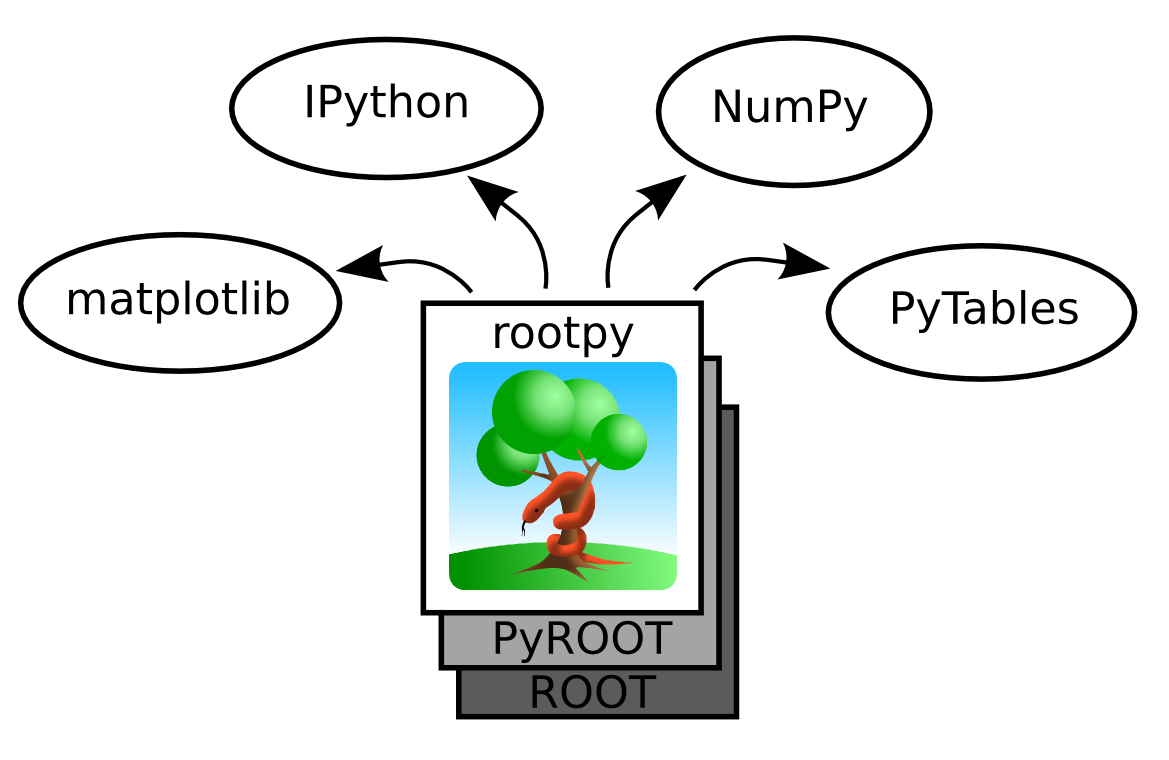
\includegraphics[height=.7\textheight]{figs/rootpy-map.png}
    \end{center}
}

\frame{
    \frametitle{rootpy: Design \& Philosophy}

    \begin{itemize}
        \item rootpy does not aim to reproduce ROOT in Python
        but rather provide a layer on top of PyROOT that integrates more
        naturally with Python:
        \vspace{.2cm}
        \begin{itemize}
            \itemsep=.2cm
            \item Setting and getting parameters with simple attributes:\\
                {\bf hist.linecolor = 'darkseagreen'}
            \item Simple navigation through TFiles:\\
                {\bf hist = myfile.somedirectory.otherdirectory.histname}
            \item Support for Python exceptions and logging
            \item Python has a garbage collector but C++ does not: leads to
                strange issues in PyROOT. rootpy addresses these problems.
            \item Arithmetic operators that are otherwise not implemented in
                PyROOT are implemented in rootpy
        \end{itemize}
    \end{itemize}
}

\frame{
    \frametitle{rootpy: Design \& Philosophy}

    \begin{itemize}
        \itemsep=.2cm
        \item rootpy classes simply inherit from the corresponding ROOT classes
            and may override methods to add functionality or be decorated with
            additional attributes
        \item rootpy classes typically have the same name as ROOT classes with
            the T removed
            but instead of having many histogram classes rootpy has three: Hist,
            Hist2D, Hist3D with a type argument in the constructor that controls
            which ROOT.THX is inherited from.
        \item Anywhere Python is typically slow (looping) is instead compiled as a C extension
            module. rootpy provides very fast conversion of ROOT Trees into
            NumPy arrays as well as efficiently filling ROOT histograms with
            NumPy arrays.

    \end{itemize}
}

\begin{frame}[fragile]
    \frametitle{rootpy: Installation}
    
    \begin{center}
        {\bf Come to the tutorial at 2pm today}
    \end{center}

    \begin{enumerate}
        \itemsep=.3cm
        \item First install ROOT with python support enabled (PyROOT)
        \item Clone the rootpy repository with git:\\\vspace{.3cm}
            \hspace{1cm} {\bf git clone git://github.com/rootpy/rootpy.git}
        \item or checkout with svn:\\\vspace{.3cm}
            \hspace{1cm} {\bf svn checkout http://svn.github.com/rootpy/rootpy}
        \item Install:\\\vspace{.3cm}
            \hspace{1cm} {\bf cd rootpy}\\
            \hspace{1cm} {\bf python setup.py install --user}
        \item See the
                \href{https://github.com/rootpy/rootpy/blob/master/README.rst}{README} on github for full instructions.
    \end{enumerate}
\end{frame}

\begin{frame}[fragile]
    \frametitle{rootpy example: opening a TFile}
    \begin{footnotesize}
\begin{minted}{python}
from rootpy.testdata import get_file

# use the test file shipped with rootpy
with get_file() as f:
    # access objects by name as properties of the current dir
    myhist = f.dimensions.hist2d
    # recursively walk through the file
    for path, dirs, objects in f.walk():
        # do something
        print path, dirs, objects
\end{minted}
\end{footnotesize}

\end{frame}

\begin{frame}[fragile]
    \frametitle{rootpy example: creating histograms}
    \begin{footnotesize}
    \begin{footnotesize}
\begin{pyglist}[language=python,texcl=true,abovecaptionskip=0,style=vs,bgcolor=Moccasin]
from ROOT import TH3D
from array import array

# variable width bins
hist3d = TH3D('3d', '3d', 3, array('d', [0, 3, 10, 100]),
                          5, array('d', [2.3, 4.2, 5.8, 10, 20, 25.5]),
                          2, array('d', [-100, 0, 20]))
# ROOT is missing some constructors... (the following will not work)
hist3d = TH3D('3d', '3d', 3, 0, 5,
                          5, array('d', [2.3, 4.2, 5.8, 10, 20, 25.5]),
                          2, array('d', [-100, 0, 20]))
\end{pyglist}
\end{footnotesize}

    \end{footnotesize}
\end{frame}

\begin{frame}[fragile]
    \frametitle{rootpy example: filling a TTree}
    \begin{footnotesize}
    \begin{footnotesize}
\begin{pyglist}[language=python,texcl=true,abovecaptionskip=0,style=vs,bgcolor=Moccasin]
from array import array
from random import gauss

output_file = TFile.Open('output.root', 'recreate')
some_float = array('f', [0.])
some_int = array('i', [0])
tree = TTree('mytree', '')
tree.Branch('some_float', some_float, 'some_float/F')
tree.Branch('some_int', some_int, 'some_int/I')

for i in xrange(100):
    some_float[0] = gauss(0, 1)
    some_int[0] = i
    tree.Fill()

tree.Write()
output_file.Close()
\end{pyglist}
\end{footnotesize}

    \end{footnotesize}
\end{frame}

\frame{
    \frametitle{Summary}
    
    \begin{itemize}
        \item Python is a very powerful language for high-level analysis
        \item rootpy provides a more pythonic way of using ROOT in Python and
            the freedom to interface with a large and growing collection of very
            powerful scientific python packages.
    \end{itemize}
    \begin{block}{Outlook}
    \begin{itemize}
        \item rootpy is still a work in progress many new features are currently
            under development.
        \item Python 3 is becoming more mainstream -- support for this in rootpy
            will be required.
        \item Better integration with the IPython prompt: full tab completion
            and addition of helpful builtin commands like pylab.
        \item ROOT 6 will be coming out very soon. Cling will replace CINT.
            See this recent
            \href{http://indico.cern.ch/contributionDisplay.py?contribId=255&confId=149557}{talk at CHEP}.
            PyROOT and hence rootpy will hopefully benifit from these major
            ROOT developments. 
        \item Improve our online documentation and tutorials.
        \item Maybe someday an officially supported extension of ROOT?
    \end{itemize}
    \end{block}
}

\frame{
    \begin{center}
        \begin{Huge}
            rootpy
        \end{Huge}
    \end{center}
    \begin{itemize}
        \itemsep=.3cm
        \item See the documentation:
            \href{http://www.rootpy.org}{http://www.rootpy.org}
        \item Contribute on Github:
            \href{https://github.com/rootpy/rootpy}{https://github.com/rootpy/rootpy}
    \end{itemize}
}

%\frame{
%    \begin{center}
%    \begin{Huge}
%        EXTRAS
%    \end{Huge}
%    \end{center}
%}

%\frame{
%    \frametitle{CINT vs rootpy}
%
    % table of comparisons
    % opening a file
    % getting a histogram from the file
    % looking at bin contents
    % setting style attributes
    % reading a tree  
%}

\end{document}
